\subsection{Deformations in Nematic Order: Free Energy}
As we've seen so far, it's useful to understand the free energy it takes to deform the order parameter. We'll imagine a completely ordered state, such that changes in the nematic order are only the result of changes in the angle. It is possible to develop the elements in the free energy phenomenologically from symmetry. In the nematic case we find three elements.

\begin{figure}[!htb]
    \centering
    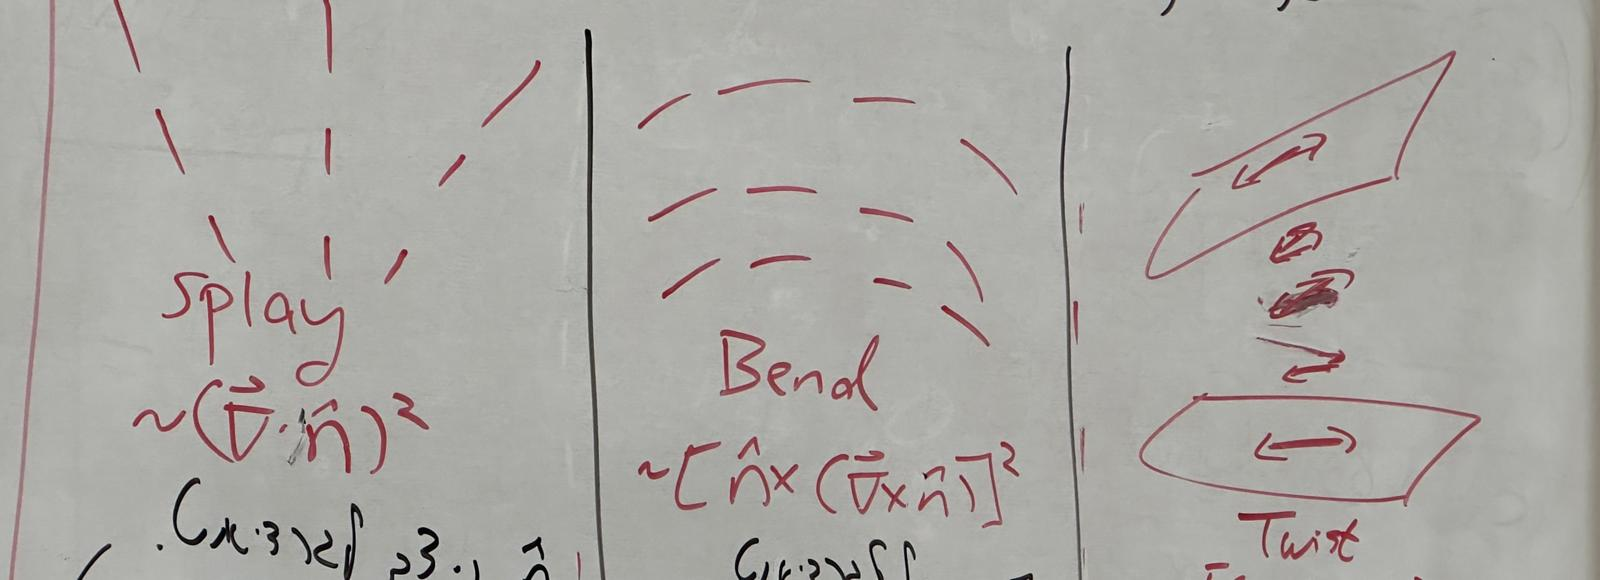
\includegraphics[width=1\textwidth]{images/nematic_deformations.jpg}
\end{figure}

\begin{description}
    \item[Splays] The elements have the form \(\sim\ins{\nabla \cdot \hat{n}}^2\).\  \(\hat{n}\) is perpendicular to the gradient and \(\delta\hat{n}\) is parallel to the gradient.
    \item[Bends] The elements have the form \(\ins{\hat{n}\times\ins{\nabla\times\hat{n}}}^2\).\  \(\hat{n}\) is parallel to the gradient and \(\delta\hat{n}\) is perpendicular ot the gradient.
    \item[Twists] This is only defined in three dimensions. The elements have the form \(\ins{\hat{n}\cdot\ins{\nabla\times\hat{n}}}^2\). Both \(\hat{n}\) and \(\delta\hat{n}\) are perpendicular to the gradient.
\end{description}
in each of the cases the element \(\hat{n}\) appears an even number of times and the derivatives are of second order. In total, the deformation energy we find is called the Frank Free Energy or the Frank Elasticity:
\begin{equation}
    F = \int \dd \vec{r} \frac{1}{2}\ins{K_1\ins{\nabla\cdot\hat{n}}^2+K_2\ins{\hat{n}\cdot\ins{\nabla\times\hat{n}}}^2+K_3\ins{\hat{n}\times\ins{\nabla\times\hat{n}}}^2}
\end{equation}
the coefficients \(K_{1,2,3}\) are called the Frank coefficients and in general they have different values but are of similar order of magnitude. For simplicity it is possible to assume \(K_1=K_2=K_3\). This is called the `one-constant approximation' in which case it is then possible to express the free energy as
\begin{equation}
    F = \int \dd \vec{r} \frac{K}{2}\partial_\alpha n_\beta\partial_\alpha n_\beta = \int\dd \vec{r} \frac{K}{2}\ins{\nabla\hat{n}}^2
\end{equation}
in practice the final expression has another boundary element called the sadlle-splay. We'll return to the active current \(-\Lambda\partial_\beta Q_{\alpha\beta}\) in 2D. We'll look at how a current can result from a splay or a bend.
\newpage
\begin{figure}[!htb]
    \centering
    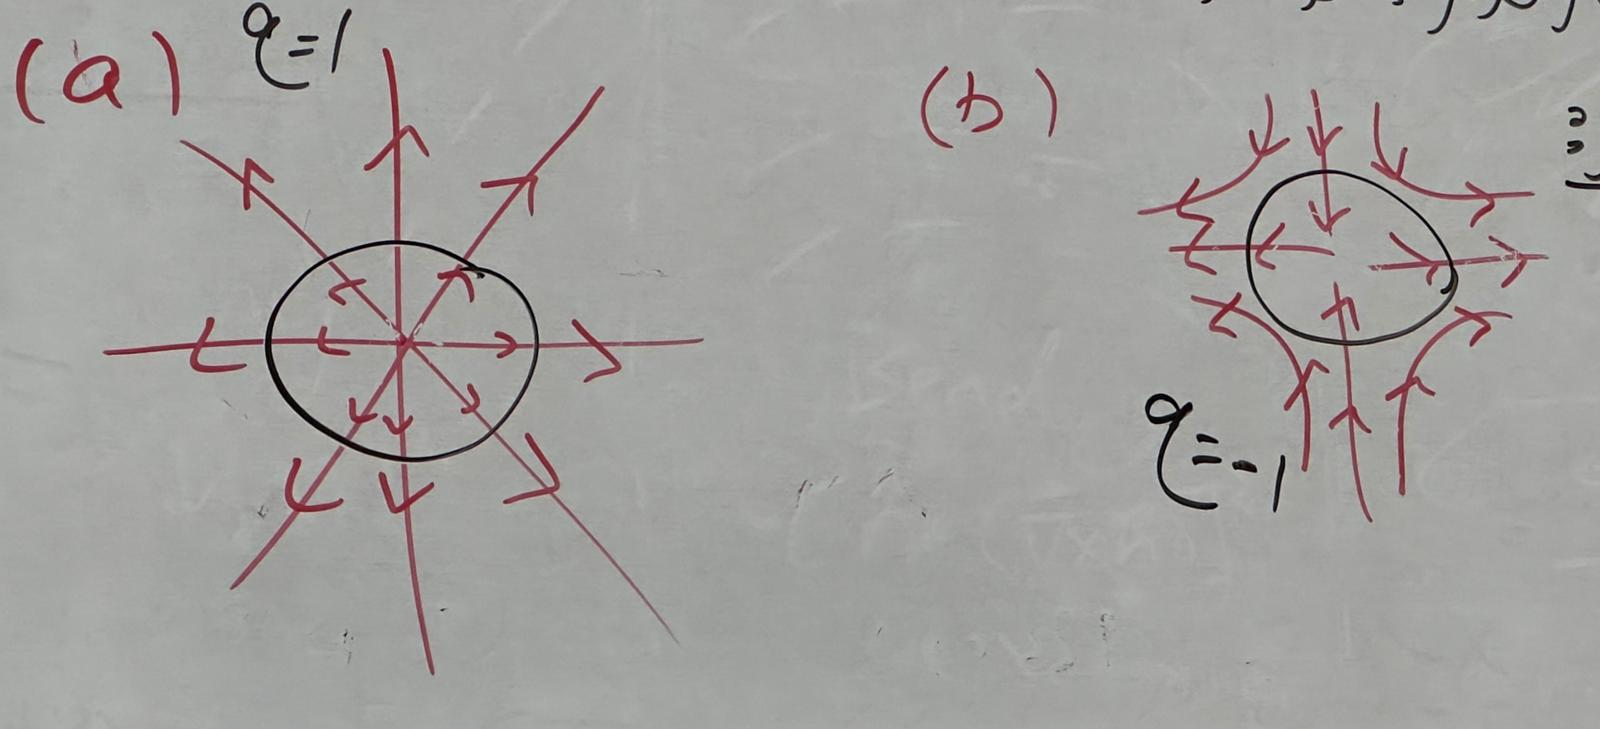
\includegraphics[width=0.5\textwidth]{images/polar_deformations.jpg}
\end{figure}
It is possible to think of each line as a force dipole. When they are non-homogenous there are regions which will contribute to the creation of a total force (like electric dipoles and charge). For case 1 in the above figure:
\begin{align}
    \hat{n} = \hat{r} \implies \partial_\beta\ins{n_\alpha n_\beta} = n_\alpha\partial_\beta n_\beta + \cancel{n_\beta \partial_\beta n_\alpha} = 2\hat{r}
\end{align}
and for case 2:
\begin{align}
    \hat{n} = \hat{\theta} \implies \partial_\beta\ins{n_\alpha n_\beta} = \cancel{n_\alpha\partial_\beta n_\beta} + n_\beta\partial_\beta n_\alpha = \frac{1}{r}\partial_\theta\ins{-\sin\theta,\cos\theta} = -\frac{\hat{r}}{r}
\end{align}
\section{Topological Defects (in 2D)}
Unlike the deformations we saw already, there are deformations with singularities in the direction \(\hat{r}\), i.e places where the direction is undefined. Such deformations are called topolotical defects. We'll focus on them in 2 dimensions. It is possible to characterize defects by the `topological charge' q. It is called as the winding number. We'll assume that \(\hat{n} = \ins{\cos\theta,\sin\theta}\). In that case the topological charge is given by
\begin{equation}
    \boxed{\oint\dd\theta = 2\pi q}
\end{equation}
\begin{wrapfigure}[15]{r}{0.5\textwidth}
    \centering
    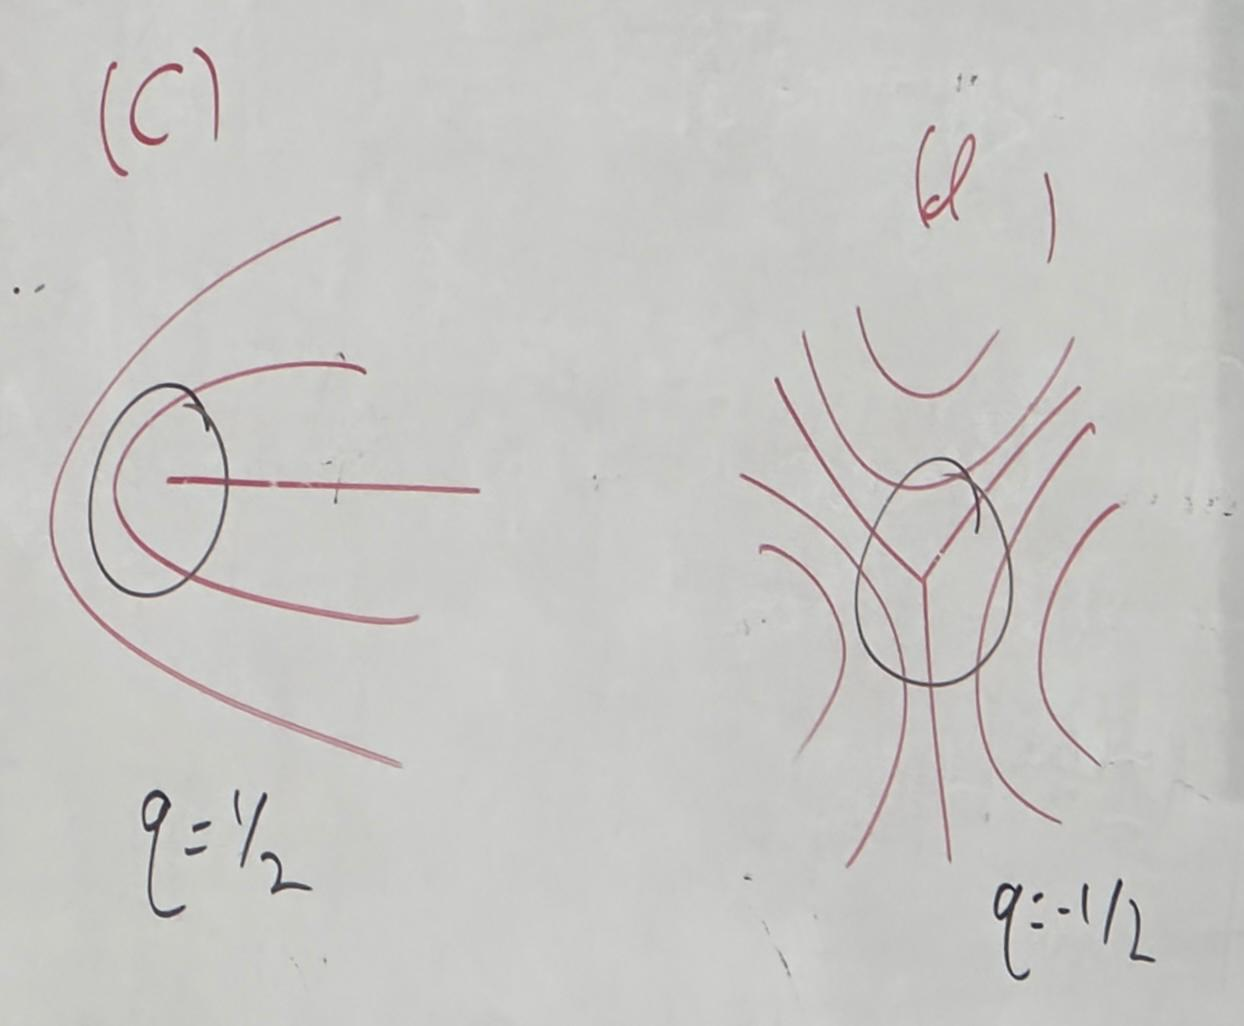
\includegraphics[width=0.5\textwidth]{images/nematic_defects.jpg}
\end{wrapfigure}
where the integral is over any closed path which encloses the defect and its direction is counter-clockwise. For polar order, \(q\) is a whole number. A couple notes:
\begin{itemize}
    \item The value of q is independent of the path.
    \item If there are two or more defects enclosed by the path, \(q\) will be the total charge.
\end{itemize}
\subsection{The Free Energy of a Defect}
We'll employ the Frank free energy with the one-constant approximation
\begin{equation}
    F = \frac{1}{2}\int\dd^2 r K \ins{\nabla n}^2 = \frac{1}{2}\int\dd \vec{r} K\ins{\nabla\theta}^2
\end{equation}
this is analogous to electrostatics where the angle plays the rule of the electric potential and the defect will be like a charge. The configuration of \(\theta\) around the defect results from a minimization of the free energy:
\begin{equation}
    0 = \frac{\delta F}{\delta \theta} = -K\nabla^2\theta
\end{equation}
This is a local minimum. The global minimum is a constant zero. We'll solve the laplace equation we found in polar coordinates:
\begin{align}
    0 = \frac{1}{r}\partial_r\ins{r\partial_r\theta}+\frac{1}{r^2}\partial_{\phi\phi}\theta
\end{align}
Assuming that \(\theta = \theta(\phi)\)
\begin{align}
    \theta = \theta_0 + a\phi
\end{align}
We'll enforce the charge:
\begin{align}
    2\pi q = \oint\dd\theta = \int\limits_0^{2\pi}\dd\phi\diff{\theta}{\phi} = 2\pi a
\end{align}
i.e
\begin{equation}
    \boxed{\theta = \theta_0+q\phi}
\end{equation}
Now let's calculate the free energy:
\begin{align}
    \nabla\theta = \frac{q}{r}\hat{\phi} &\implies F = \int\limits_0^\infty\dd r r \int\limits_0^{2\pi}\frac{1}{2}K\frac{q^2}{r^2}\dd \phi \\
    = \pi Kq^2\int\limits_0^\infty\frac{\dd r}{r} &\implies F = \pi \left.Kq^2\ln r \right\vert_0^\infty
\end{align}
this diverges at both limits! At the limit going to infinity, this is a manufactured divergence since the system will have a finite size \(R\). At the limit of \(r=0\), our theory isn't applicable to short distances (hydrodynamic continuum theorey). We also assumed the order parameter is of magnitude 1 with only the direction changing, because of the energetic cost to change the magnitude. But close to \(r=0\), changing the direction costs so much energy that the order parameter will prefer to shrink. The solution to this problem is that we'll define a `core' of radius \(a\) such that there's an \(F_{core}\) which we can't calculate exactly, and we'll take \(a\) as the lower limit of the integral. Therefore
\begin{align}
    \boxed{F = F_{core} + \pi Kq^2\ln\frac{R}{a}}
\end{align}
like in electrostatics, the energy goes with \(q^2\). This means that we'll often find defects with the smallest \(q\) possible in equilibrium (\(\pm 1\) for polar, \(\pm 1/2\) for nematic). Moreover, defects with opposite charges will attract and will eventually merge to minimize the free energy. The result \(F \sim \ln\frac{R}{a}\) is very important in the theory of condensed matter. The entropy of the location of defects also goes \(\sim\ln\frac{R}{a}\). This gives us \(F\sim \ins{\frac{\pi K}{4}-k_B T}\ln\frac{K}{q}\). At sufficiently high temperatures defects will begin to form. This is the basis for topological phase transitions (KT/KTHN). The topology of the system has influence on the total charge of the defects (The poincare-Hopf theorem) in particular, a nematic field on the surface of a sphere must have a total topological charge \(q=2\).
\subsection{Dynamics of Active Nematic Defects}
We defined in active nematic matter a current
\begin{equation}
    j_\alpha^a = -\Lambda\partial_\beta Q_{\alpha\beta}
\end{equation}
we'll examine this element for defects \(q = \pm 1/2\). Intuition: from a simple look at the defects, \(q=1/2\) seems to have a directionality, and \(q=-1/2\) doesn't, so only the first will move.